
\documentclass[12pt, a4paper]{article}
\usepackage[utf8]{inputenc}
\usepackage{fontenc}
\usepackage{xcolor}
\usepackage{hyperref}
\usepackage[english]{babel}
\usepackage[inline]{enumitem}
\usepackage{graphicx}
\usepackage{cleveref}

\graphicspath{ {res/} }

\newcommand{\versionmajor}{0}
\newcommand{\versionminor}{1}
\newcommand{\versionpatch}{0}
\newcommand{\version}{\versionmajor.\versionminor.\versionpatch}

\title{\LARGE
    Rustfields \\ 
    \small
    Risk Analysis
    }

\author{
    Angela Cortecchia \\ 
    \small 
    angela.cortecchia@studio.unibo.it
    \and
    Paolo Penazzi \\ 
    \small
    paolo.penazzi@studio.unibo.it
}

\date{\small }

\begin{document}
\maketitle
\par\noindent\rule{\textwidth}{0.5pt}

\begin{figure}[ht]
    \centering % Centra l'immagine
    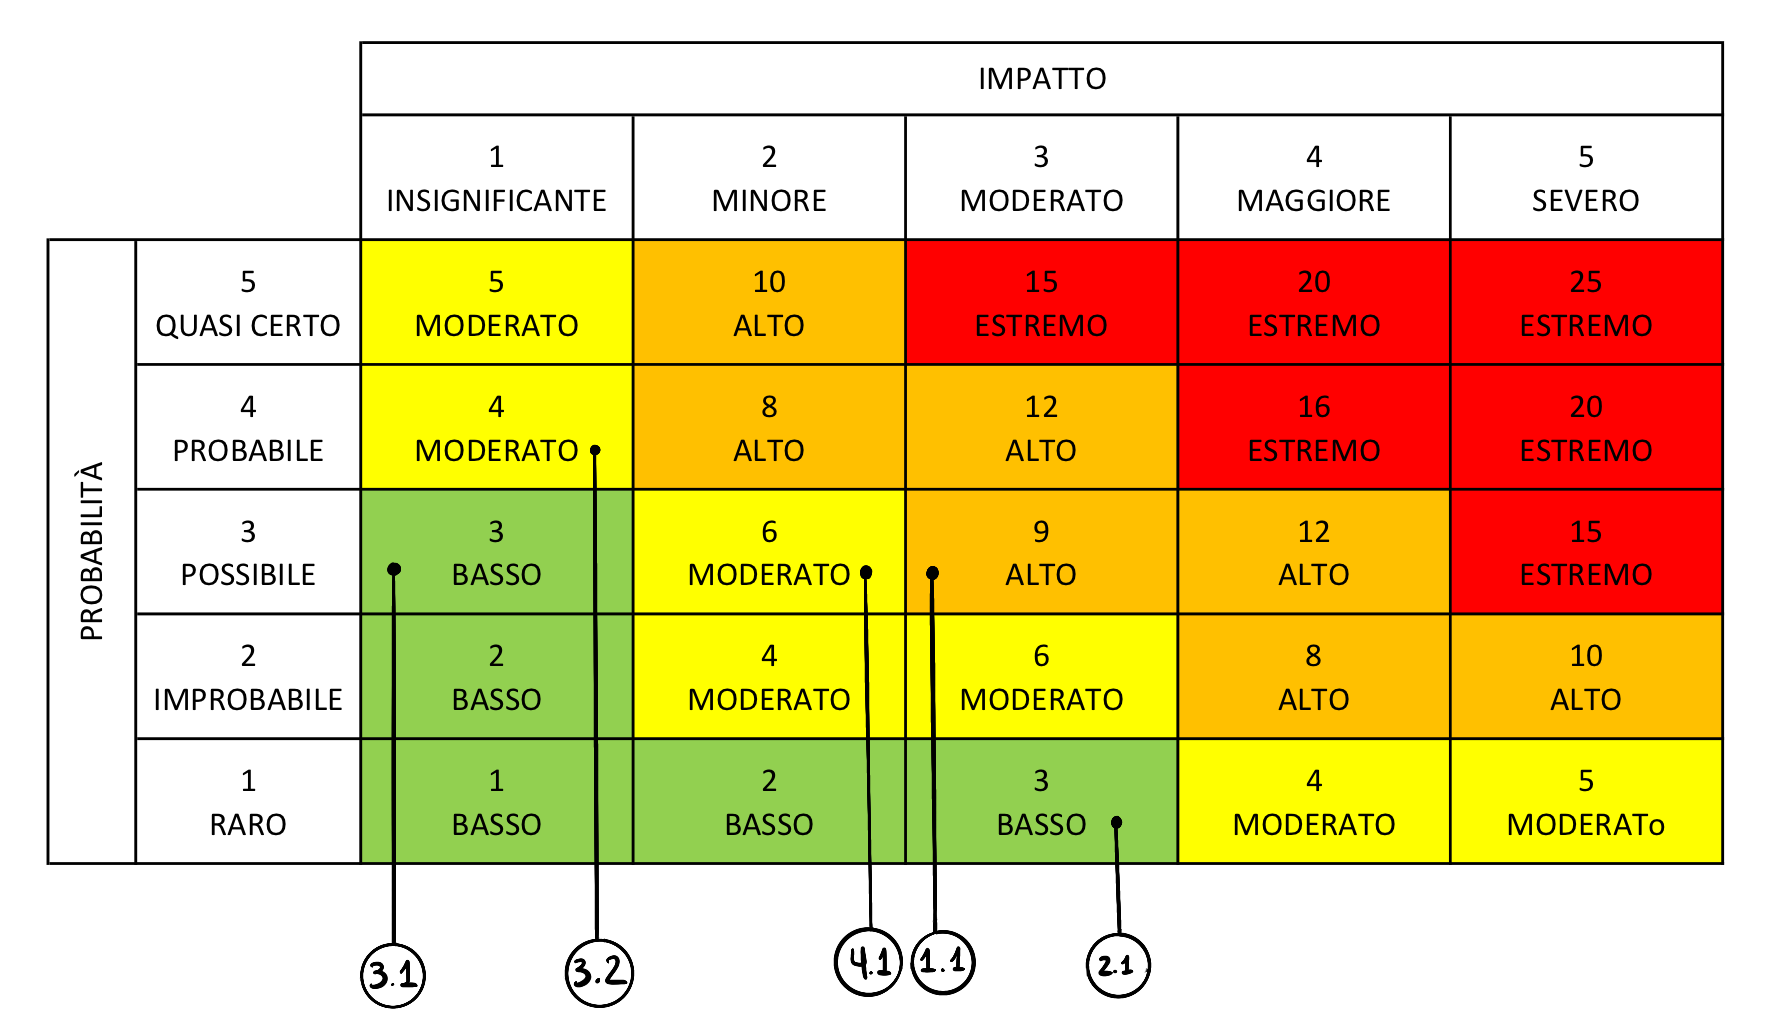
\includegraphics[width=1\linewidth]{images/risk_matrix.png}
    \caption{Matrice di rischio}
    \label{fig:matrix}
\end{figure}

\section{Rischi tecnici}
\subsection{Complessità tecnica}
\textbf{Descrizione}: La creazione di una struttura complessa potrebbe portare a ritardi.\\
\textbf{Probabilità}: Possibile(3)\\
\textbf{Impatto}:  Moderata(3)\\
\textbf{Risultato}: Alto(9)\\

\section{Rischi di Project Management}
\subsection{Complessità di integrazione con altri progetti}
\textbf{Descrizione}: Una gestione insufficiente dei sottoprogetti può causare problemi durante le fasi di integrazione tra le diverse unità.\\
\textbf{Probabilità}: Raro(1)\\
\textbf{Impatto}: Moderato(3)\\
\textbf{Risultato}: Basso(3)\\

\section{Rischi di Organizzazione}
\subsection{Mancanza di budget}
\textbf{Descrizione}: Poiché il prodotto non è stato commissionato e rientra quindi nella categoria dei progetti interni, non sono stati stabiliti limiti di budget conosciuti.\\
\textbf{Probabilità}: Possibile(3)\\
\textbf{Impatto}: Insignificante(1)\\
\textbf{Risultato}: Basso(3)\\

\subsection{Mancanza di risorse umane}
\textbf{Descrizione}: Poiché il prodotto non è stato commissionato e rientra quindi nella categoria dei progetti interni, non si può garantire un impegno costante da parte del team.\\
\textbf{Probabilità}: Probabile(4)\\
\textbf{Impatto}: Insignificante(1)\\
\textbf{Risultato}: Moderato(4)\\

\section{Rischi Esterni}
\subsection{Evoluzione delle tecnologie}
\textbf{Descrizione}: La creazione di una struttura complessa potrebbe portare a ritardi.\\
\textbf{Probabilità}: Possibile(3)\\
\textbf{Impatto}: Minore(2)\\
\textbf{Risultato}: Moderato(6)\\


\end{document}